\documentclass[aps,prd,twocolumn,superscriptaddress,nofootinbib,longbibliography,floatfix,amsmath,amssymb,10pt]{revtex4-2}

\usepackage[T1]{fontenc}
\usepackage{mathptmx}
\usepackage{amsthm}
\usepackage{graphicx}
\usepackage{booktabs}
\usepackage{xcolor}
\usepackage{enumitem}
\usepackage[colorlinks=true,linkcolor=blue!50!black,citecolor=blue!50!black,urlcolor=blue!50!black,bookmarksnumbered=true,hypertexnames=false]{hyperref}
\usepackage{orcidlink}
\usepackage{microtype}
\usepackage{xurl}

\makeatletter
\AtBeginDocument{\def\NAT@bibsetup{\setlength{\labelwidth}{\z@}%
 \setlength{\labelsep}{0.5em}\setlength{\itemindent}{\z@}%
 \setlength{\listparindent}{\z@}\setlength{\topsep}{\z@}%
 \setlength{\parsep}{\z@}\NATx@bibsetup}}
\let\write@bibliographystyle\relax
\let\bibliography@latex\@gobble
\makeatother

\tolerance=2000
\emergencystretch=2em
\hbadness=2000
\hfuzz=1pt

\newtheorem{theorem}{Theorem}
\newtheorem{lemma}[theorem]{Lemma}
\newtheorem{proposition}[theorem]{Proposition}
\newtheorem{corollary}[theorem]{Corollary}
\newtheorem*{theoremA}{Theorem A}
\newtheorem*{theoremB}{Theorem B}
\newtheorem*{theoremC}{Theorem C}
\newtheorem*{theoremD}{Theorem D}
\newtheorem*{theoremE}{Theorem E}
\theoremstyle{definition}
\newtheorem{definition}[theorem]{Definition}
\theoremstyle{remark}
\newtheorem{remark}[theorem]{Remark}

\newcommand{\R}{\mathbb{R}}
\newcommand{\C}{\mathbb{C}}
\newcommand{\N}{\mathbb{N}}
\newcommand{\E}{\mathbb{E}}
\renewcommand{\P}{\mathbb{P}}
\newcommand{\Gbar}{\overline{G}}
\newcommand{\dd}{\mathrm{d}}
\newcommand{\cut}{\C\setminus(-\infty,0]}
\DeclareMathOperator{\re}{Re}
\DeclareMathOperator{\im}{Im}
\DeclareMathOperator{\Var}{Var}
\DeclareMathOperator{\PV}{PV}
\DeclareMathOperator*{\esssup}{ess\,sup}

\setlength{\emergencystretch}{3em}
\begin{document}

\title{Ghosts in Poisson Brane Gases}

\author{Deep Bhattacharjee\,\orcidlink{0000-0003-0466-750X}}
\email{itsdeep@live.com}
\thanks{$*$\,Corresponding author. Second address:
\nolinkurl{d.bhattacharjee@erl-forschung.de}.}
\affiliation{Formerly, Electro-Gravitational Space Propulsion Laboratory
(EGSPL), Bhubaneswar, Odisha 751030, India}
\affiliation{Formerly, University of Calcutta, Senate House, 87/1 College
Street, Kolkata 700073, West Bengal, India}

\author{Ushashi Bhattacharya\,\orcidlink{0009-0002-2254-3914}}
\email{rai.bhattacharya.in@gmail.com}
\affiliation{Formerly, National Taiwan University, Taipei 106319, Taiwan}

\date{21 October 2026}

\begin{abstract}
\itshape
A Poisson gas of branes with mass intensity $\nu$ dresses the graviton
propagator by the random entire function $\prod_k(1+p^2/t_k)$. We prove that
the gas average of the propagator equals
$p^{-2}\exp[-\int p^2\nu(\dd t)/(p^2+t)]$, so that the massive states carry
total weight $e^{-\nu(0,\infty)}-1<0$. For $\nu=\lambda(t)\,\dd t/t$ the
averaged spectrum consists of ghosts alone exactly when $\lambda\le1$, and
every average with a finite four-dimensional tadpole has states of both
signs. Frozen gases keep alternating residues.
\par\medskip\upshape\noindent
\textit{2020 Mathematics Subject Classification.} Primary 81T15, 60G55;
Secondary 30D15, 44A15, 30E25, 83C45.
\end{abstract}

\keywords{Poisson point process; Laguerre--P\'olya class; complete Bernstein
function; ghost}

\maketitle

\makeatletter
\renewcommand\l@subsection[2]{}
\renewcommand\l@subsubsection[2]{}
\makeatother
\tableofcontents

\section{Introduction}\label{sec:intro}

Einstein gravity quantized around flat space is not renormalizable, and the
two ways of improving its ultraviolet behaviour pull against each other. A
kinetic operator $p^2a(p^2)$ with $a$ a polynomial of degree $n$ makes the
propagator fall like $p^{-2-2n}$, but it also gives the propagator $n$ massive
poles, and their residues add up to $-1$, so at least one of them describes a
state of negative norm, a ghost~\cite{Stelle1977,AsoreyLopezShapiro1997}.%
\footnote{The sum rule is the partial-fraction identity
$1/(z\prod_{j=1}^n(1+z/t_j))=1/z+\sum_k r_k/(z+t_k)$ evaluated against the
behaviour at infinity: since the left side decays like $z^{-1-n}$ with
$n\ge1$, the coefficient of $1/z$ in the expansion at infinity vanishes, and
that coefficient is $1+\sum_kr_k$. When the masses are distinct and ordered,
$t_1<\dots<t_n$, the residue $r_k$ has the sign $(-1)^k$, so the lightest
massive state is always a ghost and the ghosts and healthy states alternate.
This is the content of Proposition~\ref{prop:residues} below, there for
infinitely many masses.} Replacing the polynomial by an entire function
without zeros, $a=e^{H}$, removes the extra poles while keeping a fast decay
in Euclidean momenta; this is the route of Efimov, Krasnikov, Kuz'min,
Tomboulis, Biswas, Mazumdar, Siegel and Modesto~\cite{Efimov1967,Krasnikov1987,Tomboulis1997,BiswasMazumdarSiegel2006,BGKM2012,Modesto2012,ModestoRachwal2014}.
The price is that the entire function has to be chosen by hand.

A brane gas offers a mechanism that produces form factors rather than
postulating them~\cite{SinghaRoy2025,Bhattacharjee2022,BCGarchive}. A
graviton that crosses a brane of mass scale $t$ picks up a factor $1+p^2/t$
in its kinetic operator, and a configuration $\Pi=\{t_1<t_2<\cdots\}$ of
branes turns the free propagator $1/p^2$ into
\begin{equation}\label{eq:G}
G_\Pi(z)=\frac{1}{zF_\Pi(z)},\qquad F_\Pi(z)=\prod_k\Bigl(1+\frac{z}{t_k}\Bigr),
\qquad z=p^2.
\end{equation}
For a Poisson gas the product is a random entire function of genus zero with
negative zeros, an element of the Laguerre--P\'olya class~\cite{Levin1964}.
Each zero is a pole of the propagator, so a frozen configuration has the same
alternating residues as a polynomial form factor. The natural hope is that
averaging over the gas removes them: the expectation $\E F_\Pi(z)=\exp(z\int
t^{-1}\nu(\dd t))$ is an exponential and has no zeros at all. But
$1/(z\E F_\Pi)$ is not the expectation of any propagator. The two-point
function of a field in a random background averages to $\E G_\Pi$, and the
average of the reciprocal is not the reciprocal of the average.

This paper computes $\E G_\Pi$ exactly and reads off its spectrum. The setting
is a Poisson process $\Pi$ on $(0,\infty)$ with intensity measure $\nu$,
subject to
\begin{equation}\label{eq:H}
\int_{(0,\infty)}\min(1,t^{-1})\,\nu(\dd t)<\infty,\tag{H}
\end{equation}
which is exactly the condition under which the product~\eqref{eq:G}
converges. We write $|\nu|=\nu(0,\infty)\in(0,\infty]$ and
\begin{equation}\label{eq:phi}
\varphi(z)=\int_{(0,\infty)}\frac{z}{z+t}\,\nu(\dd t),\qquad z\in\cut .
\end{equation}

\begin{theoremA}[Theorem~\ref{thm:average}]
For every $z\in\cut$ the propagator is integrable and
\begin{equation}\label{eq:main}
\Gbar(z):=\E\,G_\Pi(z)=\frac{e^{-\varphi(z)}}{z}.
\end{equation}
\end{theoremA}

The function $\varphi$ is a complete Bernstein function~\cite{SSV2012}, so
$x\Gbar(x)=e^{-\varphi(x)}$ decreases from $1$ at $x=0$ to $e^{-|\nu|}$ at
$x=\infty$. A positive K\"all\'en--Lehmann
representation~\cite{Kallen1952,Lehmann1954} would force $x\Gbar(x)$ to
increase. Hence:

\begin{theoremB}[Theorem~\ref{thm:nopositive}]
If $\nu\neq0$, then $\Gbar$ has no representation $c/z+\int\mu(\dd
s)/(z+s)$ with $c\ge0$ and $\mu\ge0$. The graviton pole keeps residue $1$, and
the massive states carry total weight $e^{-|\nu|}-1<0$.
\end{theoremB}

The sign of the spectrum is decided by one number. Write
$\nu(\dd t)=\lambda(t)\,\dd t/t$, so that $\lambda(t)$ is the number of
branes per unit of $\log t$ near $t$.

\begin{theoremC}[Theorem~\ref{thm:threshold}]
If $\lambda\le1$ almost everywhere, then
$\Gbar(z)=1/z-\int\sigma(\dd s)/(z+s)$ with $\sigma\ge0$ of total mass
$1-e^{-|\nu|}$: every massive state in the averaged propagator is a ghost. If
$\lambda$ is continuous and locally H\"older, the spectral density is
\begin{equation}\label{eq:rho}
\rho(s)=-\frac{e^{-\re\varphi(-s+i0)}\,\sin\pi\lambda(s)}{\pi s},
\end{equation}
and it is nowhere positive if and only if $\sup\lambda\le1$.
\end{theoremC}

The same number controls the ultraviolet behaviour of the average, and the
two requirements cannot be met together.

\begin{theoremD}[Theorem~\ref{thm:tradeoff}, Corollary~\ref{cor:tadpole}]
If $\Lambda=\esssup\lambda<\infty$, then $x\Gbar(x)\ge
e^{-\nu(0,a]}(1+x/a)^{-\Lambda}$ for all $a,x>0$. Consequently the
$D$-dimensional tadpole $\int\Gbar(p^2)\,\dd^Dp$ diverges whenever
$D\ge2+2\Lambda$; in particular it diverges in four dimensions when
$\lambda\le1$, and for continuous locally H\"older $\lambda$ a finite
four-dimensional tadpole forces the spectral density to take both signs.
\end{theoremD}

Frozen configurations behave in the opposite way. Every infinite
configuration gives a propagator that decays faster than any power, so every
Euclidean graph of a massive scalar with polynomial vertices converges
(Proposition~\ref{prop:frozenfinite}). Its poles, however, stay.

\begin{theoremE}[Theorems~\ref{thm:scalefree}, \ref{thm:notaverageable}]
For the scale-free gas $\nu=\theta\,\mathbf 1_{[t_0,\infty)}(t)\,\dd t/t$,
almost surely the residues alternate in sign starting with a ghost, sum to
$-1$, and satisfy $\log|r_k|=-(1+o(1))\,k^2/(2\theta)$. For every
absolutely continuous $\nu$ and every set $A$ with $\nu(A)>0$, the expected
total residue $\E\sum_k|r_k|\mathbf 1_A(t_k)$ is infinite.
\end{theoremE}

The last statement explains why Theorem~A cannot be obtained by averaging the
pole expansion term by term: the residues have no mean, and the smooth
spectrum~\eqref{eq:rho} appears only after the propagator itself is averaged.

\subsection{What is proved and what is not}

Every theorem, proposition and lemma of this paper is proved here by hand,
without conditions beyond those stated. The results concern the propagator,
that is, the tree-level two-point function. They say that for the
multiplicative brane gas neither the frozen nor the averaged propagator is
free of ghosts, and that in the averaged theory the cancellation of
ultraviolet divergences and the positivity of the spectrum exclude each other
in the precise sense of Theorem~D. Nothing here proves ultraviolet finiteness
or ultraviolet completeness of quantum gravity, and nothing addresses
unitarity of the interacting theory; Sec.~\ref{sec:discussion} states what
remains open. The archive~\cite{BCGarchive} took the propagator of the
averaged gas to be $1/(z\E F_\Pi)$; Theorem~A replaces it by the average of
the propagator, which is the quantity that enters correlation functions.

\begin{figure*}[t]
\centering
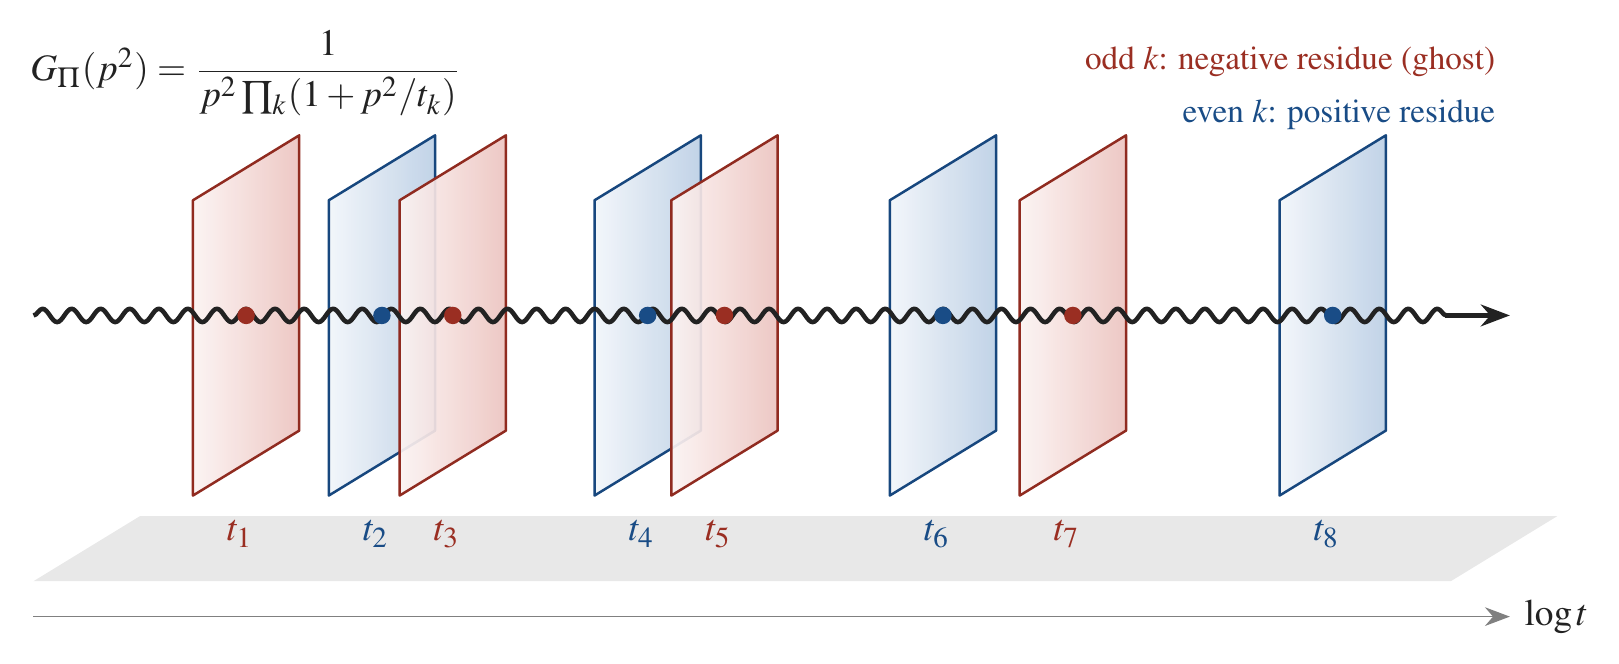
\includegraphics[width=0.94\textwidth]{figures/fig_stack.png}
\caption{A frozen brane gas. Each brane of mass scale $t_k$ multiplies the
graviton kinetic operator by $1+p^2/t_k$, so the propagator has a pole at
$p^2=-t_k$. Ordering the masses increasingly, the residue at $-t_k$ is
negative for odd $k$ and positive for even $k$
(Proposition~\ref{prop:residues}); the lightest massive state is a ghost.
The horizontal axis is $\log t$, the coordinate in which the scale-free gas
of Theorem~\ref{thm:scalefree} is a homogeneous Poisson process.}
\label{fig:stack}
\end{figure*}

\subsection{History}\label{sec:history}

Field theories with higher derivatives were studied by Pais and
Uhlenbeck~\cite{PaisUhlenbeck1950}, who saw that the extra poles of the
propagator come with alternating signs. Lee and Wick~\cite{LeeWick1969} tried
to keep such theories unitary by moving the ghost poles off the real axis, and
the modern form of this idea is Anselmi and Piva's fakeon
prescription~\cite{AnselmiPiva2017}. Stelle~\cite{Stelle1977} showed that
gravity with curvature-squared terms is renormalizable and has a massive
spin-two ghost. The spectral representation of a two-point function in terms
of a positive measure is due to K\"all\'en~\cite{Kallen1952} and
Lehmann~\cite{Lehmann1954}; positivity of that measure is the statement that
the states created by the field have positive norm.\footnote{For a scalar
field $\phi$ with $\langle0|\phi|0\rangle=0$, the K\"all\'en--Lehmann
representation reads $\langle0|T\phi(x)\phi(0)|0\rangle=\int_0^\infty
\Delta_F(x;s)\,\mu(\dd s)$ with $\Delta_F(x;s)$ the Feynman propagator of mass
$\sqrt s$ and $\mu$ a positive measure, because $\mu(\dd s)$ is the norm of
the projection of $\phi(0)|0\rangle$ onto states of invariant mass squared
$s$. In Euclidean momentum space this is $G(p^2)=\int\mu(\dd s)/(p^2+s)$.
A measure that is negative on a set of masses signals states of negative norm
there, which is what the word ghost means in this paper. A discrete negative
term $-1/(p^2+m^2)$ is a ghost particle of mass $m$; a negative density is a
continuum of them.}

Efimov~\cite{Efimov1967} introduced nonlocal interactions with entire form
factors, and Krasnikov~\cite{Krasnikov1987}, Kuz'min, Tomboulis~\cite{Tomboulis1997}
and Biswas, Mazumdar and Siegel~\cite{BiswasMazumdarSiegel2006} applied the
idea to gauge theories and gravity. Biswas, Gerwick, Koivisto and
Mazumdar~\cite{BGKM2012} showed that an exponential form factor removes the
Newtonian singularity, and Modesto~\cite{Modesto2012} and Modesto and
Rachwa{\l}~\cite{ModestoRachwal2014} constructed super-renormalizable and
finite theories along these lines. Shapiro~\cite{Shapiro2015} observed that
the dressed propagator of such theories can develop complex poles, and
Briscese, Calcagni, Modesto and Nardelli~\cite{Briscese2024} analysed when a
nonlocal propagator has a K\"all\'en--Lehmann representation. Power counting
for Euclidean graphs rests on Weinberg's theorem~\cite{Weinberg1960}.

The mathematics used here is classical. The Poisson process and the formulas
of Campbell and Mecke are in Kingman~\cite{Kingman1993} and Last and
Penrose~\cite{LastPenrose2017}. Entire functions of genus zero with real
zeros, the Laguerre--P\'olya class, are treated by Levin~\cite{Levin1964}.
Complete Bernstein functions and their characterization by the sign of the
imaginary part are in Schilling, Song and
Vondra\v{c}ek~\cite{SSV2012}.\footnote{A function $f\colon(0,\infty)\to
[0,\infty)$ is a complete Bernstein function if
$f(x)=a+bx+\int_{(0,\infty)}\frac{x}{x+s}\,\sigma(\dd s)$ with $a,b\ge0$ and
$\sigma$ a positive measure with $\int(1+s)^{-1}\sigma(\dd s)<\infty$. By
\cite[Thms.~6.2 and 6.9]{SSV2012} this holds if and only if $f$ extends
holomorphically to $\cut$, satisfies $\im f(z)\ge0$ whenever $\im z>0$, and
has a finite limit $f(0+)$. Then $a=f(0+)$, $b=\lim_{x\to\infty}f(x)/x$,
and $\sigma$ is recovered from the boundary values of $\im f$ on the
negative axis. The class is closed under many operations; the one used in
Theorem~\ref{thm:threshold} is that a nonnegative bounded holomorphic function
whose imaginary part has the sign of $\im z$ is a Stieltjes transform of a
finite positive measure up to the constant and the linear term.} The boundary
values of Cauchy integrals are given by the formulas of
Plemelj~\cite{Plemelj1908} and Privalov, in the form of
Muskhelishvili~\cite{Muskhelishvili1953}. Our earlier work on brane gases and
on quantum gravity~\cite{SinghaRoy2025,Bhattacharjee2022,BCGarchive} is the
physical motivation.

\section{The gas and its frozen propagator}\label{sec:frozen}

\subsection{Setting}

Throughout, $\nu$ is a Radon measure on $(0,\infty)$ satisfying~\eqref{eq:H},
and $\Pi$ is a Poisson process with intensity $\nu$. Condition~\eqref{eq:H}
says that $\nu(0,1]<\infty$ and $\int_{(1,\infty)}t^{-1}\nu(\dd t)<\infty$,
so $\nu$ is finite on bounded sets but may have infinite total mass.

\begin{lemma}\label{lem:product}
Almost surely $\Pi\cap(0,b]$ is finite for every $b$, and
$\sum_{t\in\Pi}\min(1,t^{-1})<\infty$. On this event $F_\Pi$ is an entire
function, $F_\Pi(x)\ge1$ for $x\ge0$, and the zeros of $F_\Pi$ are the points
$-t$, $t\in\Pi$. If $\nu$ has no atoms, the points of $\Pi$ are almost surely
distinct and the zeros are simple.
\end{lemma}

\begin{proof}
Campbell's formula~\cite[Prop.~2.7]{LastPenrose2017} gives
\[
\E\sum_{t\in\Pi}\min(1,t^{-1})=\int\min(1,t^{-1})\,\nu(\dd t)<\infty ,
\]
so the sum is finite almost surely, and $\Pi\cap(0,b]$ has a Poisson number of
points with finite mean $\nu(0,b]$. On compact sets $|z|\le R$ we have
$\sum_{t\in\Pi}|z|/t\le R\sum_{t\in\Pi}t^{-1}<\infty$ after removing the
finitely many points in $(0,1]$, so the product converges absolutely and
uniformly there; a locally uniform limit of polynomials is entire, and an
absolutely convergent product vanishes only where a factor does. For $x\ge0$
every factor is at least $1$. If $\nu$ has no atoms, the probability that two
points coincide is zero, by the same formula applied to the second factorial
measure $\nu\otimes\nu$, which gives the diagonal measure zero.
\end{proof}

\subsection{Residues}

Assume $\nu$ has no atoms and list the points as $t_1<t_2<\cdots$. The
propagator $G_\Pi=1/(zF_\Pi)$ is meromorphic with simple poles at $0$ and at
each $-t_k$. Its residue at $0$ is $1$, and its residue at $-t_k$ is
\begin{equation}\label{eq:rk}
r_k=-\prod_{j\neq k}\Bigl(1-\frac{t_k}{t_j}\Bigr)^{-1},
\end{equation}
the product converging absolutely by Lemma~\ref{lem:product}. Denote by
$r_k^{(N)}$ the same expression with $j$ restricted to $j\le N$, for $k\le N$.

\begin{proposition}\label{prop:residues}
Let $t_1<t_2<\cdots$ be the points of a configuration with
$\sum_kt_k^{-1}<\infty$.
\begin{enumerate}[label=(\roman*),leftmargin=*,itemsep=1pt]
\item $(-1)^kr_k>0$ for every $k$. In particular $r_1<0$: the lightest massive
state is a ghost.
\item For every $N$, $\sum_{k=1}^Nr_k^{(N)}=-1$.
\item For each $k$, $|r_k^{(N)}|$ increases with $N\ge k$ and converges to
$|r_k|$, and $r_k^{(N)}$ has the sign of $r_k$.
\item If $\sum_k|r_k|<\infty$, then $\sum_kr_k=-1$.
\end{enumerate}
\end{proposition}

\begin{proof}
(i) In~\eqref{eq:rk} the factors with $j>k$ lie in $(0,1)$ and the $k-1$
factors with $j<k$ are negative, so the product has the sign $(-1)^{k-1}$ and
$r_k$ the sign $(-1)^k$.

(ii) The rational function $R_N(z)=1/(z\prod_{j\le N}(1+z/t_j))$ has simple
poles at $0$ and $-t_1,\dots,-t_N$ with residues $1$ and
$r_1^{(N)},\dots,r_N^{(N)}$, and $R_N(z)=O(|z|^{-N-1})$ at infinity. The sum
of its residues is the residue at infinity with the sign reversed, which is
the coefficient of $z^{-1}$ in the expansion of $R_N$ at infinity; it vanishes
since $N\ge1$. Hence $1+\sum_kr_k^{(N)}=0$.

(iii) Passing from $N$ to $N+1$ multiplies $r_k^{(N)}$ by
$(1-t_k/t_{N+1})^{-1}$, a number larger than $1$ because
$0<t_k<t_{N+1}$. The infinite product of these factors converges since
$\sum_jt_j^{-1}<\infty$.

(iv) By (iii), $|r_k^{(N)}|\mathbf 1_{k\le N}\le|r_k|$ and
$r_k^{(N)}\to r_k$, so dominated convergence applied to (ii) gives
$\sum_kr_k=\lim_N\sum_{k\le N}r_k^{(N)}=-1$.
\end{proof}

A frozen configuration with infinitely many branes therefore has infinitely
many ghosts, one at every odd position. Theorem~\ref{thm:scalefree} shows that
for the scale-free gas the residues decay fast enough for (iv) to apply.

\subsection{Euclidean finiteness of a frozen configuration}

The ultraviolet behaviour of a frozen configuration is as good as it can be.

\begin{proposition}\label{prop:frozenfinite}
Let $\Pi=\{t_1<t_2<\cdots\}$ be infinite with $\sum_kt_k^{-1}<\infty$.
\begin{enumerate}[label=(\roman*),leftmargin=*,itemsep=1pt]
\item For every $n$ and $x\ge0$, $F_\Pi(x)\ge x^n/(t_1\cdots t_n)$.
\item Let $m>0$ and $G_m(x)=1/((x+m^2)F_\Pi(x))$. For every connected graph
$\Gamma$ in $D$ Euclidean dimensions, with propagators $G_m(p_e^2)$ on the
internal lines, vertex factors polynomial in the momenta, and fixed external
momenta, the Feynman integral converges absolutely.
\end{enumerate}
\end{proposition}

\begin{proof}
(i) Drop the factors with $k>n$, which are at least $1$, and use
$1+x/t_k\ge x/t_k$.

(ii) By (i) with $n$ replaced by any $M$, $G_m(x)\le
C_M(1+x)^{-M}$, and $G_m\le m^{-2}$. Choose a spanning tree of $\Gamma$; the
$L$ lines outside it, the chords, carry momenta $k_i+a_i$, where
$k_1,\dots,k_L\in\R^D$ are independent loop momenta and the $a_i$ are linear
in the external momenta. The integrand is bounded by
\[
C\prod_{i=1}^L(1+|k_i|)^d\,(1+|k_i+a_i|^2)^{-M}\,m^{-2(E-L)},
\]
where $d$ is the total degree of the vertex polynomials and $E$ the number of
internal lines; the tree lines were bounded by $m^{-2}$. Each factor is
integrable over $\R^D$ once $2M>d+D$.
\end{proof}

\begin{figure*}[t]
\centering
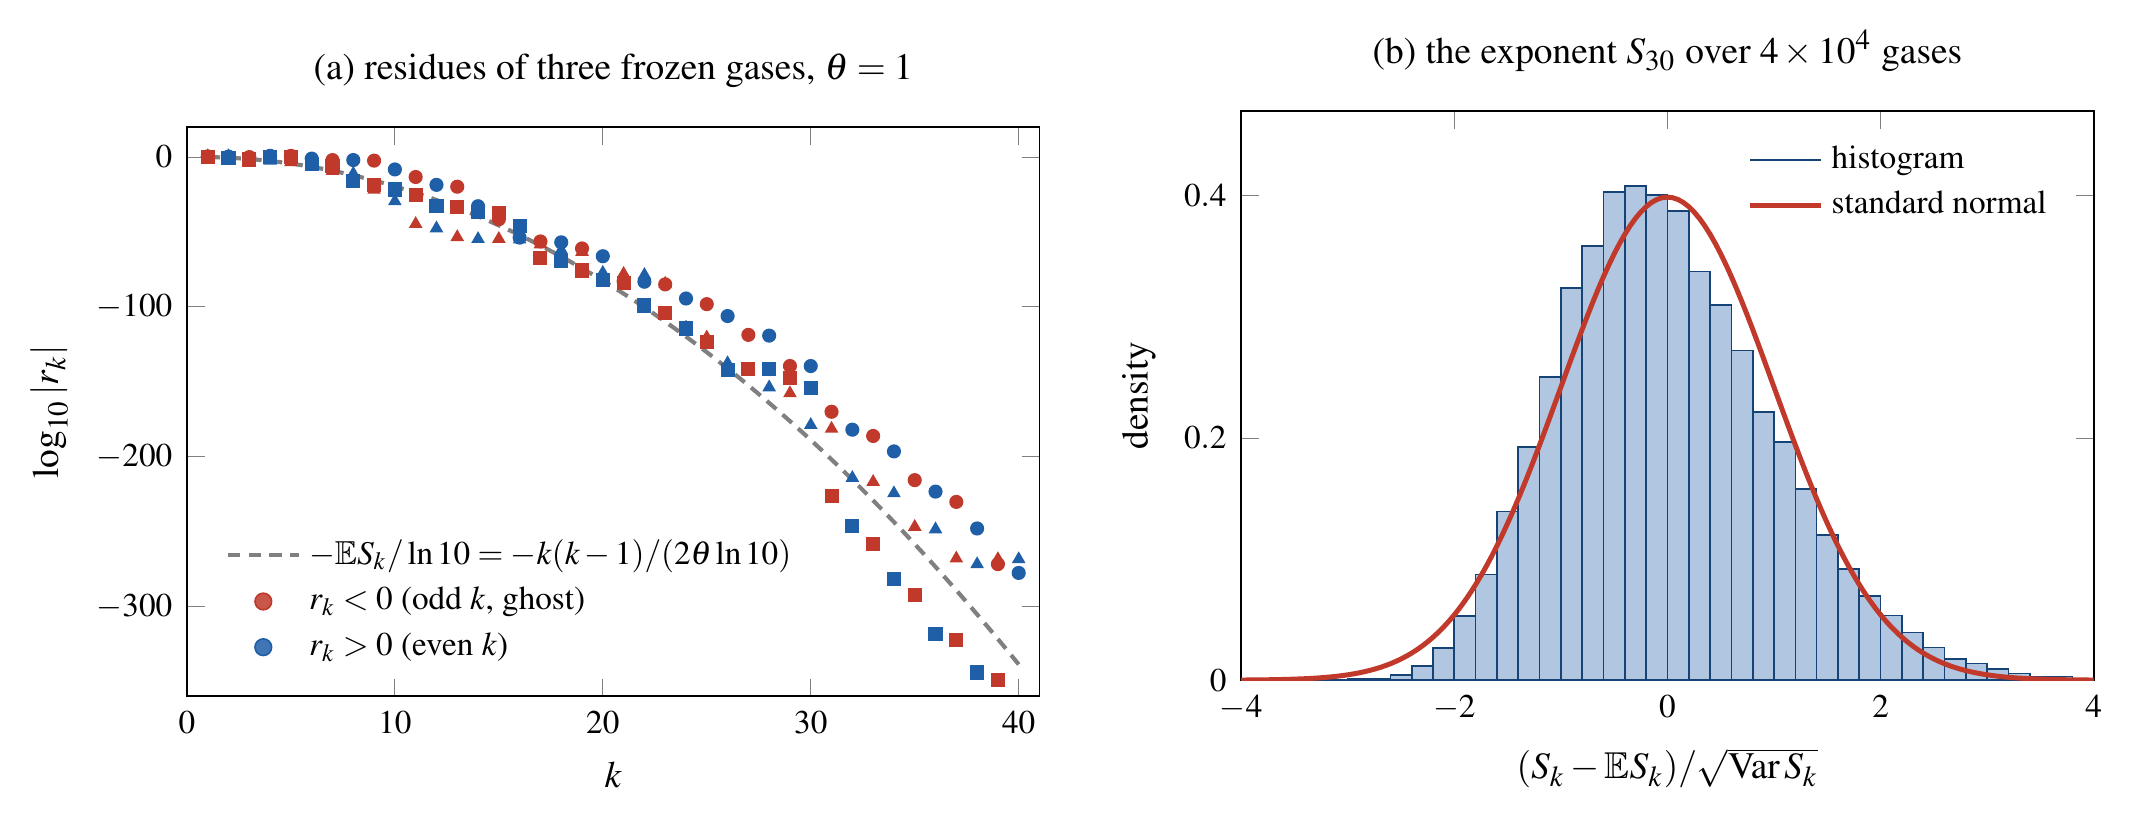
\includegraphics[width=0.96\textwidth]{figures/fig_residues.png}
\caption{(a) The residues $r_k$ of three frozen configurations of the
scale-free gas with $\theta=1$, on a logarithmic scale. Circles, squares and
triangles mark the three configurations; red marks negative residues and blue
positive ones. The dashed curve is $-\E S_k/\ln10$, the leading term of
Theorem~\ref{thm:scalefree}. (b) The exponent
$S_{30}=\sum_{i<30}i\,g_i$ over $4\times10^4$ configurations, centred and
scaled; it is a weighted sum of independent exponential gaps, and its
skewness is visible.}
\label{fig:residues}
\end{figure*}

\subsection{The scale-free gas}

Take $\nu=\theta\,\mathbf 1_{[t_0,\infty)}(t)\,\dd t/t$ with $\theta,t_0>0$.
By the mapping theorem~\cite[Thm.~5.1]{LastPenrose2017} the points are
$t_k=t_0e^{u_k}$, where $u_1<u_2<\cdots$ are the arrival times of a Poisson
process of rate $\theta$ on $[0,\infty)$. The gaps $g_k=u_{k+1}-u_k$ and
$u_1$ are independent with exponential law of mean $1/\theta$. Put
\begin{equation}\label{eq:SR}
S_k=\sum_{j<k}(u_k-u_j)=\sum_{i=1}^{k-1}i\,g_i,\qquad
R_k=-\sum_{j\neq k}\log\bigl(1-e^{-|u_j-u_k|}\bigr).
\end{equation}
The second expression for $S_k$ holds because the gap $g_i$ separates $u_j$
from $u_k$ exactly when $j\le i<k$.

\begin{theorem}\label{thm:scalefree}
For the scale-free gas, almost surely:
\begin{enumerate}[label=(\roman*),leftmargin=*,itemsep=1pt]
\item $\log|r_k|=-S_k+R_k$ for every $k$, with $R_k\ge0$;
\item $S_k=\frac{k^2}{2\theta}(1+o(1))$ and $R_k=O((\log k)^2)$ as
$k\to\infty$; in particular $\log|r_k|=-(1+o(1))k^2/(2\theta)$;
\item $\sum_k|r_k|<\infty$, so the residues alternate in sign starting with a
ghost and sum to $-1$;
\item $\log F_\Pi(x)=\frac\theta2\bigl(\log\frac x{t_0}\bigr)^2(1+o(1))$ as
$x\to\infty$.
\end{enumerate}
\end{theorem}

\begin{proof}
(i) For $j<k$, $|1-t_k/t_j|=e^{u_k-u_j}(1-e^{-(u_k-u_j)})$, and for $j>k$,
$|1-t_k/t_j|=1-e^{-(u_j-u_k)}$. Taking $-\log$ of the absolute value
of~\eqref{eq:rk} gives $-S_k+R_k$, and every term of $R_k$ is positive.

(ii) and (iv) are proved in Appendix~\ref{app:scalefree}. (iii) follows from
(ii) and Proposition~\ref{prop:residues}.
\end{proof}

The residues therefore fall off like a Gaussian in their index
(Fig.~\ref{fig:residues}), and the ghosts never thin out: the configuration
has a ghost of weight $e^{-k^2/(2\theta)(1+o(1))}$ at every odd $k$.

\subsection{Residues have no mean}

\begin{theorem}\label{thm:notaverageable}
Let $\nu(\dd t)=\lambda(t)\,\dd t/t$ with $\lambda\ge0$ locally integrable and
satisfying~\eqref{eq:H}, and let $A\subset(0,\infty)$ be a Borel set with
$\nu(A)>0$. Then
\[
\E\sum_k|r_k|\,\mathbf 1_A(t_k)=\infty .
\]
\end{theorem}

\begin{proof}
For a configuration $\pi$ and a point $t\in\pi$ let
$r_t(\pi)=-\prod_{u\in\pi\setminus\{t\}}(1-t/u)^{-1}$, the residue of
$G_\pi$ at $-t$. The Mecke formula~\cite[Thm.~4.1]{LastPenrose2017} gives
\[
\E\sum_{t\in\Pi}|r_t(\Pi)|\mathbf 1_A(t)=\int_A\E\,|r_t(\Pi\cup\{t\})|\,
\nu(\dd t),
\]
and $|r_t(\Pi\cup\{t\})|=\prod_{u\in\Pi}h_t(u)$ with
$h_t(u)=u/|u-t|$. By independence of a Poisson process on disjoint sets,
the expectation is the product of the expectations over
$\Pi\cap(0,t/2)$ and $\Pi\cap[t/2,\infty)$. The first factor is positive: it
equals $\exp(-\int_{(0,t/2)}(1-h_t)\,\dd\nu)$ by
Lemma~\ref{lem:pgfl}, and $0\le1-h_t\le1$ there. On $[t/2,\infty)$ we have
$h_t\ge1$, and the same lemma with monotone convergence gives the second
factor as $\exp(\int_{[t/2,\infty)}(h_t-1)\,\dd\nu)$, with value in
$(0,\infty]$. Since $h_t(u)\ge t/(2|u-t|)$ for $u\ge t/2$,
\[
\int_{[t/2,2t]}(h_t-1)\,\dd\nu\ge\frac14\int_{|u-t|<t/2}
\frac{\lambda(u)}{|u-t|}\,\dd u-3\int_{[t/2,2t]}\dd\nu.
\]
If $t$ is a Lebesgue point of $\lambda$ with $\lambda(t)>0$, then
$\int_{|u-t|<r}\lambda\ge\lambda(t)r$ for $r\le r_0$, and writing
$|u-t|^{-1}=r_0^{-1}+\int_{|u-t|}^{r_0}r^{-2}\dd r$ on $|u-t|<r_0$ gives
\[
\int_{|u-t|<r_0}\frac{\lambda(u)}{|u-t|}\dd u\ge
\int_0^{r_0}\frac{1}{r^2}\int_{|u-t|<r}\lambda\,\dd r\ge
\lambda(t)\int_0^{r_0}\frac{\dd r}{r}=\infty .
\]
Since $\nu(A)>0$, the set of such $t$ in $A$ has positive $\nu$-measure, and
the integral over $A$ is infinite.
\end{proof}

\section{The averaged propagator}\label{sec:average}

\begin{theorem}\label{thm:average}
Assume~\eqref{eq:H}. For every $z\in\cut$, $\E|G_\Pi(z)|<\infty$ and
$\E G_\Pi(z)=e^{-\varphi(z)}/z$, with $\varphi$ as in~\eqref{eq:phi}. The
function $\Gbar=\E G_\Pi$ is holomorphic on $\cut$.
\end{theorem}

\begin{proof}
Fix $z=|z|e^{i\alpha}$ with $|\alpha|<\pi$ and put
$g(t)=(1+z/t)^{-1}=t/(t+z)$, so that $1/F_\Pi(z)=\prod_{t\in\Pi}g(t)$. For
$t>0$,
\begin{equation}\label{eq:halfangle}
|t+z|\ge\cos(\alpha/2)\,(t+|z|),
\end{equation}
because $|t+z|^2-\cos^2(\alpha/2)(t+|z|)^2=\frac12(1-\cos\alpha)(t-|z|)^2$.
Hence $|g|\le K:=1/\cos(\alpha/2)$ and
$|1-g(t)|=|z|/|t+z|\le K\max(1,|z|)\min(1,t^{-1})$, which is
$\nu$-integrable by~\eqref{eq:H}. For $t>T:=2|z|$ we have
$|t+z|\ge t(1-|z|/t)\ge te^{-2|z|/t}$, since $1-y\ge e^{-2y}$ for $0\le
y\le\frac12$; thus $|g(t)|\le e^{2|z|/t}$. Lemma~\ref{lem:pgfl} applies and
gives $\E\prod_{t\in\Pi}g(t)=\exp(-\int(1-g)\,\dd\nu)=e^{-\varphi(z)}$, because
$1-g(t)=z/(z+t)$. The domination in that lemma is uniform for $z$ in compact
subsets of $\cut$, so $\Gbar$ is holomorphic by Morera's theorem and Fubini's
theorem.
\end{proof}

The exponent $\varphi$ has the form of a complete Bernstein function with
$a=b=0$ and $\sigma=\nu$, and~\eqref{eq:H} is equivalent to
$\int(1+t)^{-1}\nu(\dd t)<\infty$. Its basic properties are read off
from~\eqref{eq:phi}: $\varphi(0+)=0$ by dominated convergence;
$\varphi(\infty)=|\nu|$ by monotone convergence;
$\varphi'(x)=\int t(x+t)^{-2}\nu(\dd t)>0$; and
\begin{equation}\label{eq:imphi}
\im\varphi(x+iy)=\int\frac{t\,y}{(x+t)^2+y^2}\,\nu(\dd t),
\end{equation}
which has the sign of $y$.

\begin{remark}[Thinning]\label{rem:thinning}
For $x>0$, $x\Gbar(x)=e^{-\varphi(x)}$ is the probability that a thinning of
$\Pi$, keeping each point $t$ independently with probability $x/(x+t)$, has
no points. Indeed the thinned process is Poisson with intensity
$\frac{x}{x+t}\nu(\dd t)$ and total mass $\varphi(x)$. As $x$ grows the
retention probability tends to $1$ at every $t$
(Fig.~\ref{fig:thinning}(a)), and $x\Gbar(x)$ decreases to
$\P(\Pi=\emptyset)=e^{-|\nu|}$. For the scale-free gas, $x\Gbar(x)=(1+x/t_0)^{-\theta}$
is also the probability that $[t_0,t_0+x]$ contains no point of $\Pi$.
\end{remark}

\begin{remark}[Two averages]\label{rem:jensen}
The propagator of the averaged kinetic operator is $1/(z\E F_\Pi(z))=z^{-1}
\exp(-z\int t^{-1}\nu(\dd t))$ when $\int t^{-1}\nu(\dd t)<\infty$. It has no
massive poles, but it is not the average of the propagator. On the positive
axis $x/(x+t)\le x/t$ gives $e^{-\varphi(x)}\ge\exp(-x\int t^{-1}\dd\nu)$,
which is Jensen's inequality for the convex function $1/F$. The difference is
large: for the scale-free gas with $\theta=\frac32$ the first decays like
$e^{-3x/2}$ and the second only like $x^{-3/2}$
(Fig.~\ref{fig:scalefree}(b)).
\end{remark}

\begin{figure*}[t]
\centering
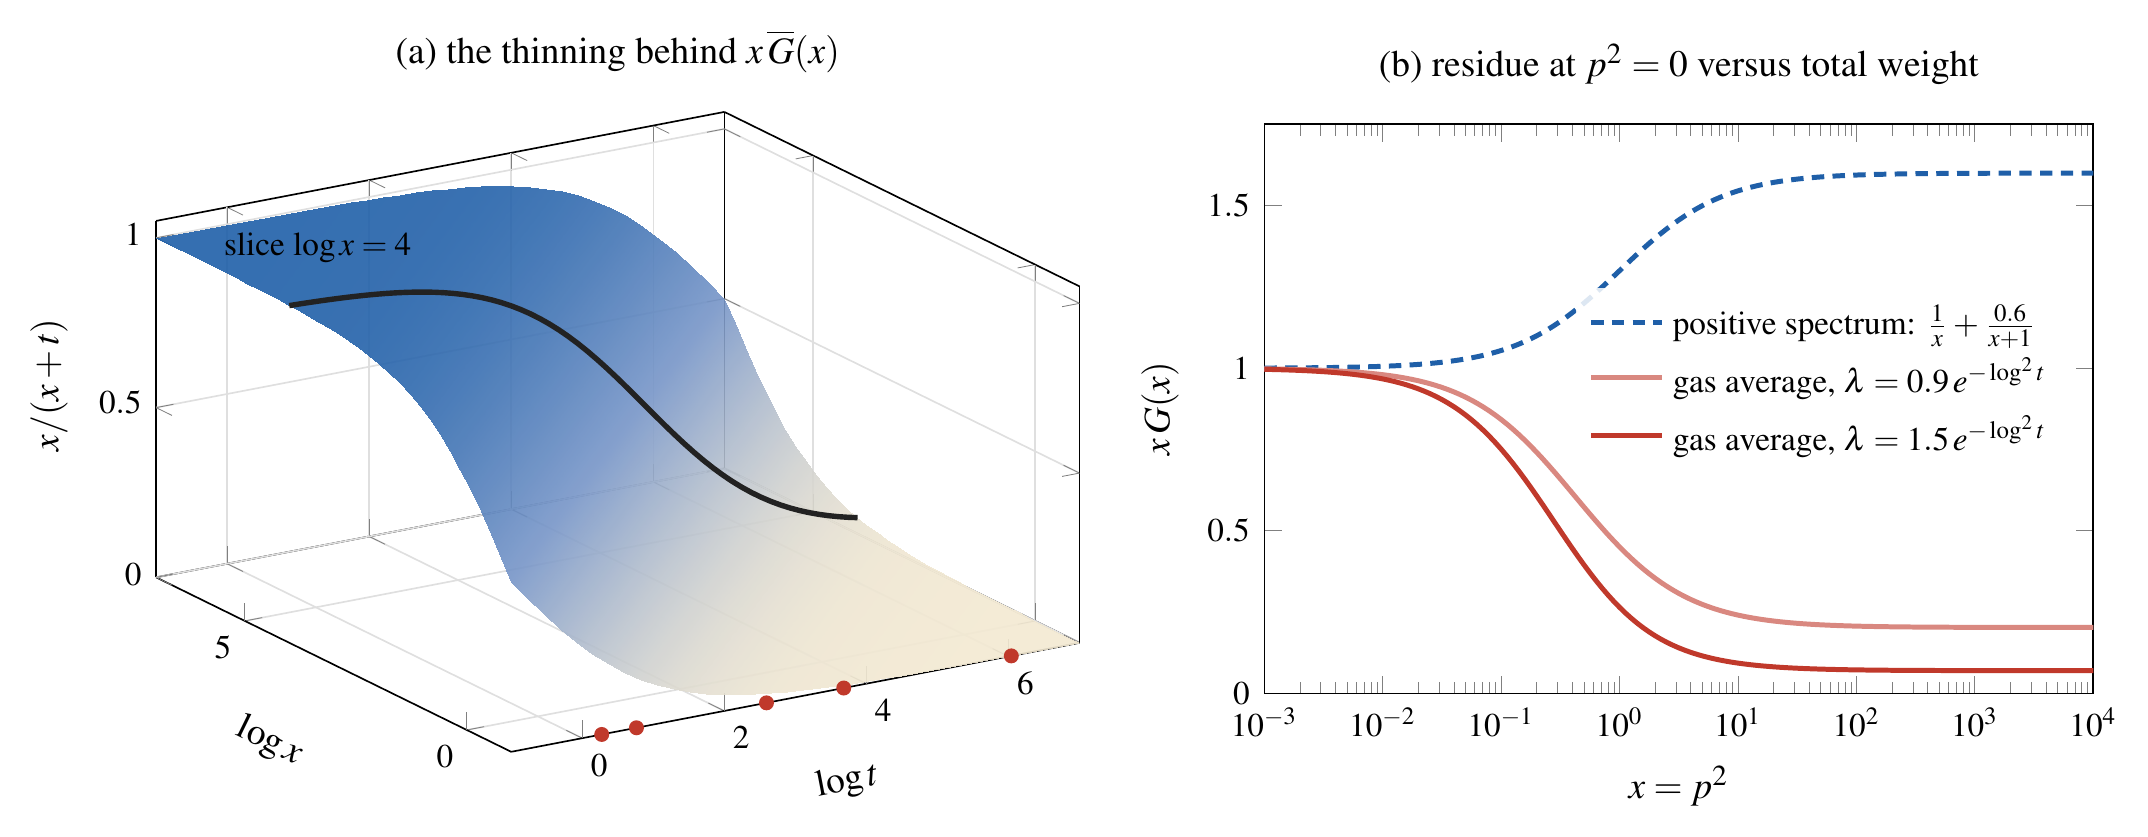
\includegraphics[width=0.96\textwidth]{figures/fig_thinning.png}
\caption{(a) The retention probability $x/(x+t)$ of the thinning in
Remark~\ref{rem:thinning}, as a surface over $(\log t,\log x)$; red dots are
the points of one configuration, and the black curve is the slice used at
$\log x=4$. The probability that no point survives is $x\Gbar(x)$. (b) For
a positive spectrum $x\,G(x)=c+\int\frac{x}{x+s}\mu(\dd s)$ increases with
$x$ (dashed). For the gas average it decreases from $1$ to $e^{-|\nu|}$
(solid), for the two intensities $\lambda=0.9\,e^{-\log^2t}$ and
$\lambda=1.5\,e^{-\log^2t}$; this is Theorem~\ref{thm:nopositive}.}
\label{fig:thinning}
\end{figure*}

\begin{theorem}\label{thm:nopositive}
Assume~\eqref{eq:H} and $\nu\ne0$. There are no $c\ge0$ and positive measure
$\mu$ on $(0,\infty)$ with $\int(1+s)^{-1}\mu(\dd s)<\infty$ such that
$\Gbar(x)=c/x+\int\mu(\dd s)/(x+s)$ for all $x>0$. Moreover
$\lim_{x\to0}x\Gbar(x)=1$ and $\lim_{x\to\infty}x\Gbar(x)=e^{-|\nu|}$.
\end{theorem}

\begin{proof}
If such a representation held, $x\Gbar(x)=c+\int\frac{x}{x+s}\mu(\dd s)$
would be nondecreasing in $x$. But $x\Gbar(x)=e^{-\varphi(x)}$ and $\varphi$ is
strictly increasing. The limits are $e^{-\varphi(0+)}$ and
$e^{-\varphi(\infty)}$.
\end{proof}

For any propagator $c/z+\int\mu(\dd s)/(z+s)$ with $\mu$ a finite signed
measure, the residue of the massless pole is $c=\lim_{x\to0}xG(x)$ and the
total massive weight is $\mu(0,\infty)=\lim_{x\to\infty}xG(x)-c$. For
$\Gbar$ these limits are $1$ and $e^{-|\nu|}-1$. The graviton keeps its
residue, and the gas contributes a net negative weight, equal to $-1$ when
$|\nu|=\infty$.

\section{The ghost threshold}\label{sec:threshold}

From now on $\nu(\dd t)=\lambda(t)\,\dd t/t$ with $\lambda\ge0$ measurable;
condition~\eqref{eq:H} reads $\int_0^1\lambda(t)t^{-1}\dd t+
\int_1^\infty\lambda(t)t^{-2}\dd t<\infty$. Then~\eqref{eq:imphi} becomes
\begin{equation}\label{eq:poisson}
\im\varphi(x+iy)=\int_0^\infty\lambda(t)\,\frac{y}{(t+x)^2+y^2}\,\dd t,
\end{equation}
the Poisson integral of $\lambda$ (extended by $0$ to $t\le0$) evaluated at
$-x+iy$. This is the reason $\lambda$, the density of branes per unit
$\log t$, is the right variable.

\begin{definition}\label{def:density}
For a function $G$ holomorphic on $\cut$, the spectral density at $s>0$ is
$\rho_G(s)=-\pi^{-1}\lim_{y\downarrow0}\im G(-s+iy)$, when the limit exists.
\end{definition}

If $G=c/z+\int\mu(\dd s')/(z+s')$ with $\mu$ a signed measure, then
$-\pi^{-1}\im G(-s+iy)=\pi^{-1}\int y((s'-s)^2+y^2)^{-1}\mu(\dd s')$, the
Poisson integral of $\mu$, and $\rho_G(s)$ is the density of $\mu$ at every
point where $\mu$ has a continuous density. A ghost continuum is a set of $s$
with $\rho_G(s)<0$.

\begin{theorem}\label{thm:threshold}
Assume~\eqref{eq:H} and $\nu(\dd t)=\lambda(t)\,\dd t/t$.
\begin{enumerate}[label=(\roman*),leftmargin=*,itemsep=1pt]
\item If $\lambda\le1$ almost everywhere, there is a positive measure $\sigma$
on $(0,\infty)$ of total mass $1-e^{-|\nu|}$ such that
\begin{equation}\label{eq:pureghost}
\Gbar(z)=\frac1z-\int_{(0,\infty)}\frac{\sigma(\dd s)}{z+s},\qquad z\in\cut .
\end{equation}
\item If $\lambda$ is H\"older continuous on a neighbourhood of $s>0$, the
limit $\varphi(-s+i0)$ exists, with
\begin{gather*}
\im\varphi(-s+i0)=\pi\lambda(s),\\
\re\varphi(-s+i0)=\PV\!\int_0^\infty\frac{-s}{t-s}\,\lambda(t)\frac{\dd t}{t},
\end{gather*}
and $\rho_{\Gbar}(s)$ is given by~\eqref{eq:rho}.
\item If $\lambda$ is continuous and locally H\"older on $(0,\infty)$, then
$\rho_{\Gbar}\le0$ on $(0,\infty)$ if and only if $\sup\lambda\le1$. If
$\sup\lambda>1$, then $\rho_{\Gbar}$ is positive on a nonempty open set and
negative on another.
\end{enumerate}
\end{theorem}

\begin{proof}
(i) If $\nu=0$ there is nothing to prove. Otherwise let $\psi=1-e^{-\varphi}$,
holomorphic on $\cut$. For $\im z=y>0$, \eqref{eq:poisson} and $\lambda\le1$
give
\[
0<\im\varphi(z)\le\int_0^\infty\frac{y\,\dd t}{(t+x)^2+y^2}
=\frac\pi2+\arctan\frac xy<\pi,
\]
so $\im\psi(z)=e^{-\re\varphi(z)}\sin\im\varphi(z)>0$. On $(0,\infty)$,
$\psi$ takes values in $[0,1)$ and $\psi(0+)=0$. By~\cite[Thms.~6.2 and
6.9]{SSV2012}, $\psi$ is a complete Bernstein function,
$\psi(x)=a+bx+\int\frac{x}{x+s}\sigma(\dd s)$ with $\sigma\ge0$. Here
$a=\psi(0+)=0$ and $b=\lim\psi(x)/x=0$ because $\psi$ is bounded. Monotone
convergence as $x\to\infty$ gives $\sigma(0,\infty)=\psi(\infty)=
1-e^{-|\nu|}$. Thus $\Gbar(x)=(1-\psi(x))/x=1/x-\int\sigma(\dd s)/(x+s)$
for $x>0$, and both sides are holomorphic on $\cut$.

(ii) With $f(t)=\lambda(t)/t$, \eqref{eq:phi} reads $\varphi(z)=-w\Phi(w)$
with $w=-z$ and $\Phi(w)=\int_0^\infty f(t)(t-w)^{-1}\dd t$, a Cauchy
integral that converges for $w\notin[0,\infty)$ by~\eqref{eq:H}. As
$z\to-s+i0$, $w\to s-i0$, and the Plemelj--Privalov
formula~\cite[\S\S16--17]{Muskhelishvili1953} gives
$\Phi(s-i0)=\PV\int f(t)(t-s)^{-1}\dd t-i\pi f(s)$, valid because $f$ is
H\"older near $s$ and integrable against $(1+t)^{-1}$ away from it. Hence
$\varphi(-s+i0)=-s\Phi(s-i0)$ has the stated real and imaginary parts.
Finally $\Gbar(-s+i0)=-s^{-1}e^{-\varphi(-s+i0)}$, so
$\im\Gbar(-s+i0)=s^{-1}e^{-\re\varphi}\sin(\pi\lambda(s))$, which
is~\eqref{eq:rho}.

(iii) If $\sup\lambda\le1$, then $\sin\pi\lambda\ge0$ and $\rho\le0$
by~\eqref{eq:rho}. Conversely let $\lambda(s_0)>1$. The integral
$\int_0^1\lambda(t)t^{-1}\dd t$ is finite, hence $\liminf_{t\to0}\lambda(t)=0$, and by
continuity $\lambda$ takes every value in $(0,\lambda(s_0))$ on $(0,s_0)$.
The open set $\lambda^{-1}(1,\min(2,\lambda(s_0)))$ is therefore nonempty, and
there $\sin\pi\lambda<0$ and $\rho>0$. The open set $\lambda^{-1}(0,1)$ is
nonempty too, and there $\rho<0$.
\end{proof}

The threshold $1$ is sharp in two senses: below it the whole massive spectrum
is a ghost continuum, and as soon as $\lambda$ crosses it somewhere, healthy
states appear but ghosts remain (Fig.~\ref{fig:spectrum}). In the window
$1<\lambda<2$ the sign of the density is positive; for larger $\lambda$ the
sign of $\sin\pi\lambda$ alternates on the intervals $(n,n+1)$, so the
averaged spectrum is a sequence of ghost and healthy bands, the continuum
counterpart of the alternating residues of Proposition~\ref{prop:residues}.

\begin{figure*}[t]
\centering
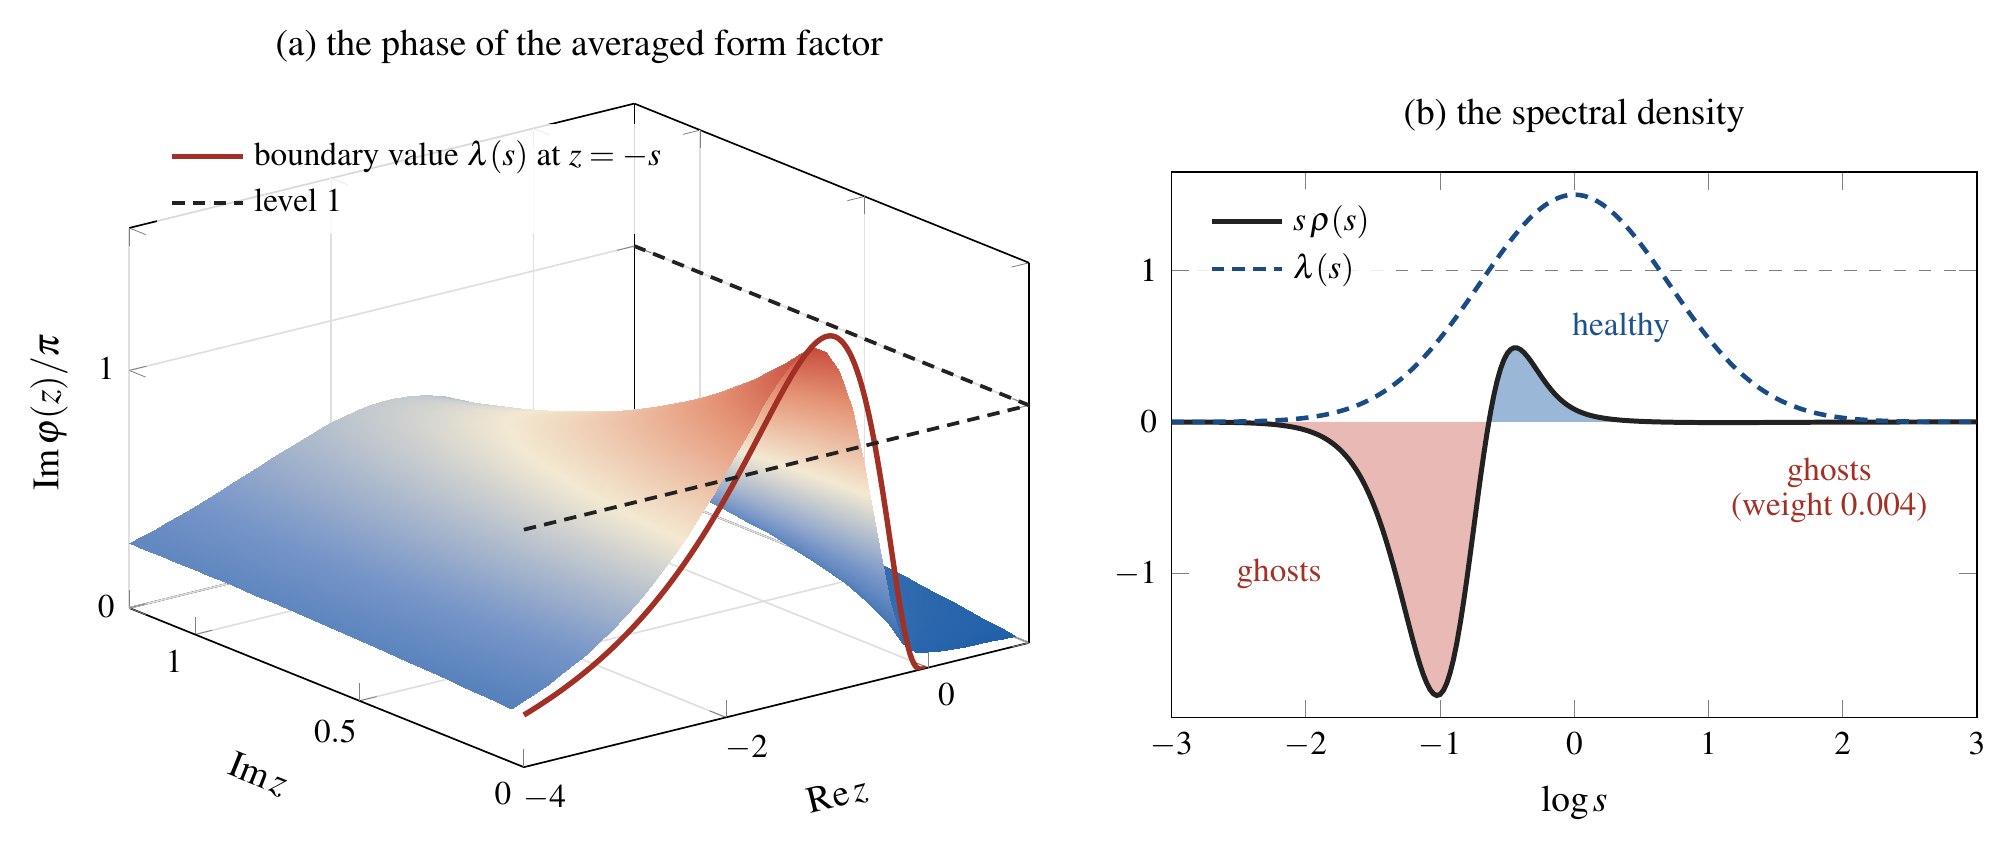
\includegraphics[width=0.96\textwidth]{figures/fig_spectrum.png}
\caption{The averaged spectrum for $\lambda(t)=1.5\,e^{-\log^2t}$. (a) The
phase $\im\varphi(z)/\pi$ over the upper half-plane. It is the Poisson
integral~\eqref{eq:poisson} of $\lambda$, and its boundary value on the cut
$z=-s$ is $\lambda(s)$ (red curve); the dashed line marks the level $1$.
(b) The spectral density $s\rho(s)$ of~\eqref{eq:rho} against $\log s$, with
$\lambda$ dashed. The density is positive exactly where $1<\lambda<2$ and
negative where $0<\lambda<1$; its integral is $e^{-|\nu|}-1=e^{-1.5\sqrt\pi}-1
\approx-0.930$, in agreement with Theorem~\ref{thm:nopositive}.}
\label{fig:spectrum}
\end{figure*}

\begin{corollary}\label{cor:scalefree}
For the scale-free gas, $\varphi(z)=\theta\log(1+z/t_0)$ and
\[
\Gbar(z)=\frac1z\Bigl(1+\frac{z}{t_0}\Bigr)^{-\theta}.
\]
\begin{enumerate}[label=(\roman*),leftmargin=*,itemsep=1pt]
\item For $0<\theta<1$, \eqref{eq:pureghost} holds with
$\sigma(\dd s)=\frac{\sin\pi\theta}{\pi}(s/t_0-1)^{-\theta}\mathbf 1_{s>t_0}
\frac{\dd s}{s}$, of total mass $1$.
\item For $\theta=1$, $\Gbar(z)=1/z-1/(z+t_0)$: a single ghost of residue
$-1$ at $t_0$.
\item For $1<\theta<2$, $\rho_{\Gbar}(s)=-\frac{\sin\pi\theta}{\pi}
(s/t_0-1)^{-\theta}s^{-1}$ is positive on $(t_0,\infty)$ and not integrable at
$t_0$.
\end{enumerate}
\end{corollary}

\begin{proof}
$\varphi(z)=\theta\int_{t_0}^\infty\frac{z\,\dd t}{t(z+t)}=
\theta\log\frac{z+t_0}{t_0}$. For $s>t_0$, $1-s/t_0+i0=(s/t_0-1)e^{i\pi}$, so
$(1+z/t_0)^{-\theta}\to(s/t_0-1)^{-\theta}e^{-i\pi\theta}$ as $z\to-s+i0$,
which gives the densities in (i) and (iii); for $0<s<t_0$ the boundary value
is real and the density vanishes. In (i), $\lambda=\theta\mathbf
1_{[t_0,\infty)}\le1$ and Theorem~\ref{thm:threshold}(i) applies; the
measure $\sigma$ there has no mass on $(0,t_0)$ and has the computed density
on $(t_0,\infty)$, and its total mass is $1=1-e^{-\infty}$. The substitution
$s=t_0(1+v)$ gives $\int\sigma=\frac{\sin\pi\theta}{\pi}\int_0^\infty
\frac{v^{-\theta}\dd v}{1+v}=\frac{\sin\pi\theta}{\pi}\cdot\frac{\pi}
{\sin\pi\theta}=1$ (Appendix~\ref{app:calc}), so $\sigma$ has no atom at
$t_0$. (ii) is the partial fraction $t_0/(z(z+t_0))=1/z-1/(z+t_0)$.
\end{proof}

At $\theta=1$ the continuum of (i) collapses into one ghost. Above it the
density is positive, yet by Theorem~\ref{thm:nopositive} the propagator is
not a positive superposition: the negative weight is concentrated at the
threshold $t_0$, where the density fails to be integrable
(Fig.~\ref{fig:scalefree}(a)).

\begin{figure*}[t]
\centering
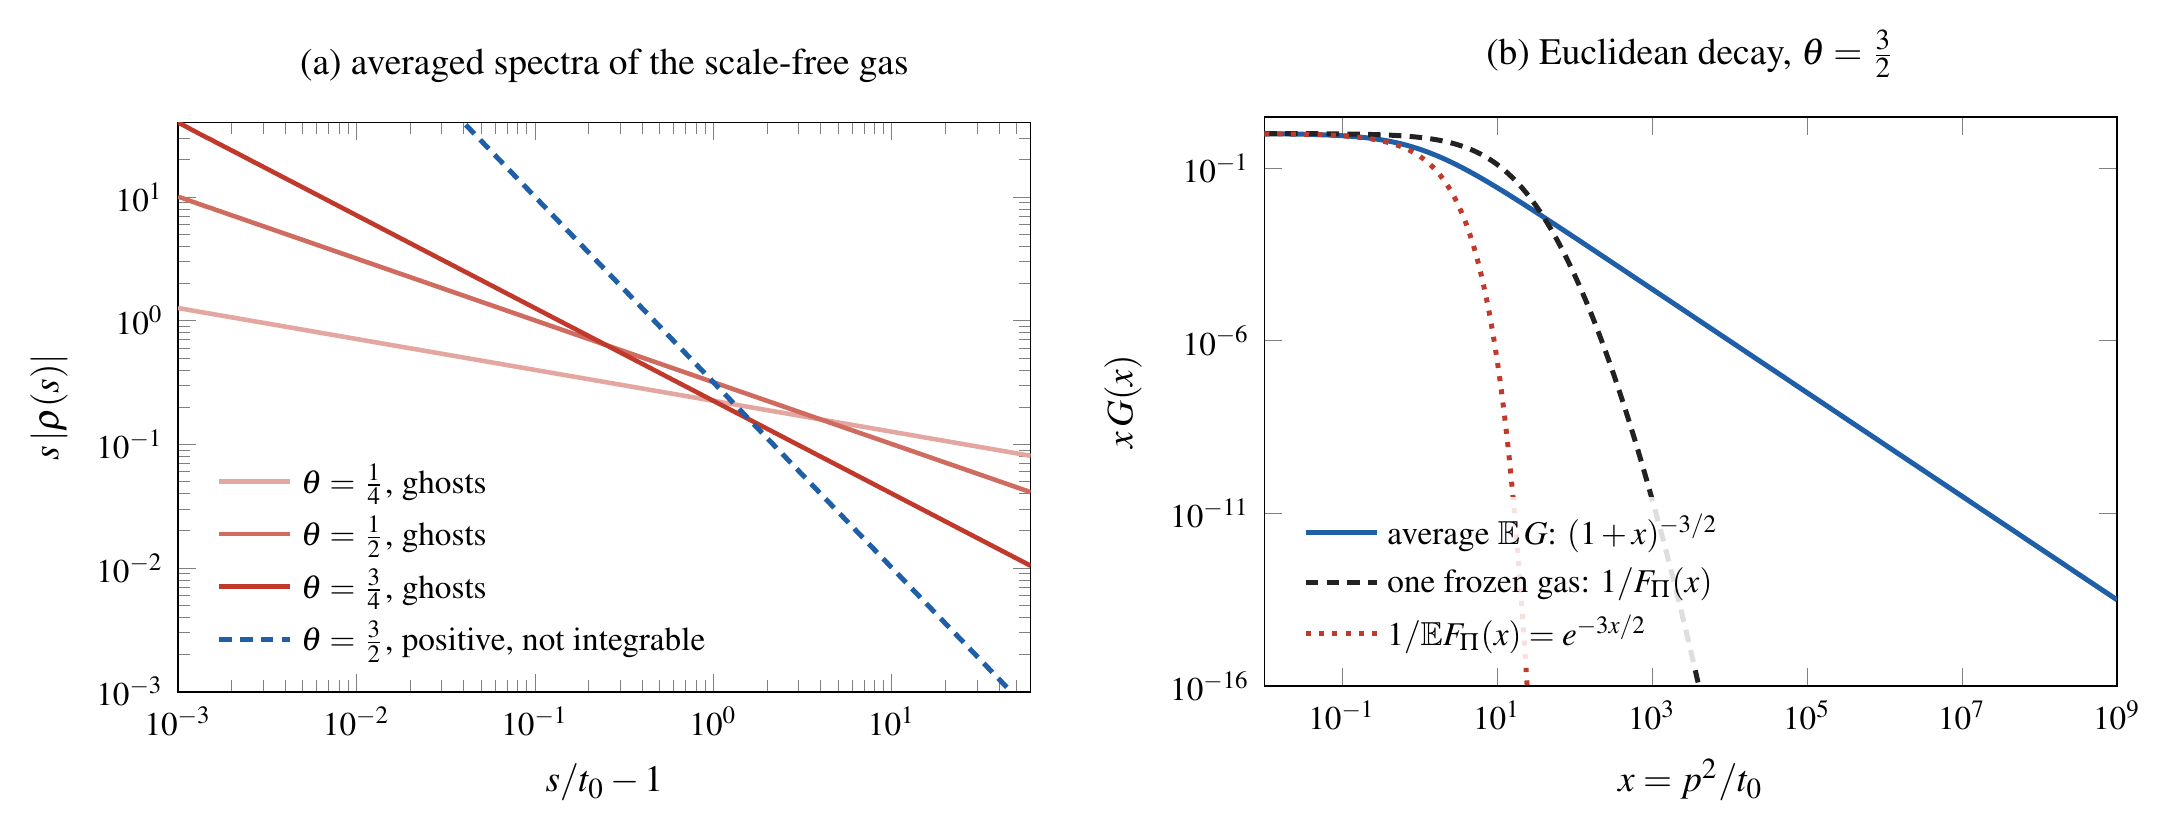
\includegraphics[width=0.96\textwidth]{figures/fig_scalefree.png}
\caption{The scale-free gas. (a) The averaged spectral density of
Corollary~\ref{cor:scalefree}, as $s|\rho(s)|$ against $s/t_0-1$: ghost
continua for $\theta=\frac14,\frac12,\frac34$, each of total weight $1$, and
for $\theta=\frac32$ a positive density that is not integrable at the
threshold. (b) Decay along the Euclidean axis for $\theta=\frac32$, $t_0=1$:
the average $x\Gbar(x)=(1+x)^{-3/2}$ (Theorem~\ref{thm:average}), one frozen
configuration $1/F_\Pi(x)$, which falls like
$\exp(-\frac34\log^2x)$ (Theorem~\ref{thm:scalefree}(iv)), and
$1/\E F_\Pi(x)=e^{-3x/2}$ (Remark~\ref{rem:jensen}).}
\label{fig:scalefree}
\end{figure*}

\section{Ultraviolet decay against positivity}\label{sec:tradeoff}

\begin{theorem}\label{thm:tradeoff}
Assume~\eqref{eq:H}, $\nu(\dd t)=\lambda(t)\,\dd t/t$ and
$\Lambda=\esssup\lambda<\infty$. For all $a,x>0$,
\[
x\Gbar(x)\ge e^{-\nu(0,a]}\Bigl(1+\frac xa\Bigr)^{-\Lambda}.
\]
\end{theorem}

\begin{proof}
Split~\eqref{eq:phi} at $a$. On $(0,a]$ the integrand is at most $1$. On
$(a,\infty)$,
\[
\int_a^\infty\frac{x}{x+t}\,\lambda(t)\frac{\dd t}{t}\le
\Lambda\int_a^\infty\Bigl(\frac1t-\frac1{x+t}\Bigr)\dd t
=\Lambda\log\Bigl(1+\frac xa\Bigr).
\]
Thus $\varphi(x)\le\nu(0,a]+\Lambda\log(1+x/a)$.
\end{proof}

For the scale-free gas with $a=t_0$ the bound is an equality, so the exponent
$\Lambda$ cannot be improved.

\begin{corollary}\label{cor:tadpole}
Under the hypotheses of Theorem~\ref{thm:tradeoff}, the tadpole
$I_D=\int_{\R^D}\Gbar(|p|^2)\,\dd^Dp$ diverges for every $D\ge2+2\Lambda$.
Hence:
\begin{enumerate}[label=(\roman*),leftmargin=*,itemsep=1pt]
\item if $\lambda\le1$, then $I_D=\infty$ for all $D\ge4$: a ghost-only
average is not ultraviolet finite at one loop in four dimensions;
\item if $\lambda$ is continuous and locally H\"older on $(0,\infty)$ and
$I_D<\infty$ for some $D\ge4$, then $\rho_{\Gbar}$ is positive on a
nonempty open set and negative on another.
\end{enumerate}
\end{corollary}

\begin{proof}
By Theorem~\ref{thm:tradeoff} with $a=1$, $\Gbar(x)\ge c\,x^{-1-\Lambda}$
for $x\ge1$, so $I_D\ge c'\int_1^\infty r^{D-3-2\Lambda}\dd r=\infty$ when
$D-2-2\Lambda\ge0$. (i) is the case $\Lambda\le1$. For (ii), if
$\Lambda=\infty$ then $\sup\lambda>1$; if $\Lambda<\infty$, finiteness of
$I_D$ forces $\Lambda>D/2-1\ge1$, and continuity gives $\sup\lambda>1$. In
both cases Theorem~\ref{thm:threshold}(iii) applies.
\end{proof}

The comparison with Proposition~\ref{prop:frozenfinite} is the main point of
this section. A frozen configuration decays faster than any power and
renders every Euclidean graph finite, at the price of infinitely many ghost
poles. Averaging trades the poles for a continuum and, in doing so, gives up
the fast decay: the average falls off only like a power, the power is the
brane density $\Lambda$, and a power large enough for a finite tadpole in
four dimensions requires a density above $1$, which brings healthy and ghost
states together. Table~\ref{tab:summary} collects the cases.

\begin{table*}[t]
\caption{The averaged propagator $\Gbar(z)=z^{-1}e^{-\varphi(z)}$ for
$\nu(\dd t)=\lambda(t)\dd t/t$. The last column refers to the tadpole
$\int\Gbar(p^2)\dd^4p$; ``finite'' requires $\esssup\lambda>1$
(Corollary~\ref{cor:tadpole}).}
\label{tab:summary}
\begin{ruledtabular}
\begin{tabular}{lllll}
Intensity & Massive spectrum & Total massive weight & Decay of $x\Gbar(x)$ & $D=4$ tadpole\\
\hline
$\lambda\le1$, $|\nu|<\infty$ & ghost continuum (Thm.~\ref{thm:threshold}) & $e^{-|\nu|}-1$ & to $e^{-|\nu|}$ & divergent\\
$\theta\mathbf 1_{[t_0,\infty)}$, $0<\theta<1$ & ghost continuum on $(t_0,\infty)$ & $-1$ & $(x/t_0)^{-\theta}$ & divergent\\
$\mathbf 1_{[t_0,\infty)}$ & one ghost at $t_0$ & $-1$ & $(x/t_0)^{-1}$ & divergent\\
$\theta\mathbf 1_{[t_0,\infty)}$, $1<\theta<2$ & positive density, singular threshold & $-1$ & $(x/t_0)^{-\theta}$ & finite\\
continuous, $\sup\lambda>1$ & both signs (Thm.~\ref{thm:threshold}(iii)) & $e^{-|\nu|}-1$ & at least $x^{-\Lambda}$ & finite only if $\Lambda>1$\\
\end{tabular}
\end{ruledtabular}
\end{table*}

\section{Discussion}\label{sec:discussion}

The results answer, for the multiplicative brane gas, the question whether
averaging over the branes removes the ghosts of a polynomial form factor. It
does not. The frozen propagator has a ghost at every odd mass
(Proposition~\ref{prop:residues}), with weights that decay like a Gaussian in
the index for the scale-free gas (Theorem~\ref{thm:scalefree}); the averaged
propagator is the explicit function~\eqref{eq:main}, whose massive spectrum
has net weight $e^{-|\nu|}-1<0$ (Theorem~\ref{thm:nopositive}) and consists
of ghosts alone whenever the gas has at most one brane per unit of $\log t$
(Theorem~\ref{thm:threshold}). The two averages of Remark~\ref{rem:jensen}
differ: the earlier claim that the averaged propagator keeps only the
graviton pole holds for $1/(z\E F_\Pi)$, which is not the average of a
propagator.

Three questions are left open. First, the averaged theory has been studied
only through its propagator. Whether a Lee--Wick or fakeon
prescription~\cite{LeeWick1969,AnselmiPiva2017} can be applied to a ghost
continuum such as~\eqref{eq:pureghost}, and what it would give for scattering
amplitudes, is not addressed here. Second, quenched and annealed averages of
loop amplitudes differ: the average of a product of propagators is not a
product of averages, and the correlations between the propagators of one
configuration are not computed in this paper. Third, the gas is
multiplicative and Poisson. Interactions between branes, or a gas whose
points repel, would change $\varphi$; the threshold argument of
Theorem~\ref{thm:threshold} uses only that $\im\varphi/\pi$ is a Poisson
integral of the brane density, and would apply to any averaged exponent of
that form.

Ultraviolet finiteness of perturbative quantum gravity is not proved here,
and the results point the other way for this model: Theorem~D shows that in
the averaged gas the decay needed for a finite four-dimensional tadpole and a
positive spectrum cannot both hold.

\section*{Data and code availability}

All proofs in this paper are by hand. The finite sum rule and sign pattern of
Proposition~\ref{prop:residues}, inequality~\eqref{eq:halfangle}, the elementary
bounds of Appendix~\ref{app:scalefree}, the bound $\im\varphi\le\pi$ used in
Theorem~\ref{thm:threshold}, the sign of~\eqref{eq:rho} in the two windows
and the partial fraction of Corollary~\ref{cor:scalefree}(ii) were also
verified in Lean~4 with Mathlib. Theorem~\ref{thm:average} was checked by
simulation, and Theorems~\ref{thm:scalefree}, \ref{thm:threshold},
\ref{thm:tradeoff} and Corollary~\ref{cor:scalefree} numerically; these
checks, in Python, C and Julia, the Lean files and the source of this paper
are in release~3.3.0 of the repository
\url{https://github.com/creelie/brane-cluster-gases}~\cite{BCGarchiveThree}.
Deep Bhattacharjee carried out the computations and the Lean, Python, C and
Julia checks with AI assistance from Claude (Anthropic); both authors approved
the final text.

\section*{Ethical declarations}

\emph{Funding.} None. \emph{Competing interests.} None.

\appendix

\section{Poisson processes}\label{app:poisson}

We use three standard facts~\cite{Kingman1993,LastPenrose2017}. Campbell's
formula: $\E\sum_{t\in\Pi}f(t)=\int f\,\dd\nu$ for measurable $f\ge0$. The
restrictions of $\Pi$ to disjoint sets are independent. The Mecke formula:
$\E\sum_{t\in\Pi}h(t,\Pi)=\int\E\,h(t,\Pi\cup\{t\})\,\nu(\dd t)$ for
measurable $h\ge0$ on pairs of a point and a configuration.

\begin{lemma}\label{lem:pgfl}
Let $g\colon(0,\infty)\to\C$ be measurable with $\int|1-g|\,\dd\nu<\infty$,
and suppose there are $T>0$, $K\ge1$ and $c\ge0$ with $|g(t)|\le K$ for
$t\le T$ and $|g(t)|\le e^{c/t}$ for $t>T$. Then $\prod_{t\in\Pi}g(t)$
converges absolutely almost surely, is integrable, and
\[
\E\prod_{t\in\Pi}g(t)=\exp\Bigl(-\int(1-g)\,\dd\nu\Bigr).
\]
If instead $g\ge1$, the same identity holds with both sides in $(0,\infty]$.
\end{lemma}

\begin{proof}
By Campbell's formula $\sum_{t\in\Pi}|1-g(t)|<\infty$ almost surely, so the
product converges absolutely. For $b>T$ the restriction $\Pi\cap(0,b]$ has a
Poisson number $N_b$ of points with mean $m_b=\nu(0,b]<\infty$, and given
$N_b=n$ the points are independent with law $\nu|_{(0,b]}/m_b$. Hence
\[
\E\!\!\prod_{t\in\Pi\cap(0,b]}\!\!g(t)=\sum_{n\ge0}e^{-m_b}\frac{1}{n!}
\Bigl(\int_{(0,b]}g\,\dd\nu\Bigr)^{\!n}
=e^{-\int_{(0,b]}(1-g)\dd\nu}.
\]
For every $b$ the partial product is bounded in modulus by
$D=K^{N_T}\exp(c\sum_{t\in\Pi,\,t>T}t^{-1})$. The two factors of $D$ are
independent, $\E K^{N_T}=e^{(K-1)\nu(0,T]}$, and by the first computation
with $g=e^{c/t}$, $\E\exp(c\sum_{t>T}t^{-1})=\exp\int_{(T,\infty)}
(e^{c/t}-1)\dd\nu\le\exp(ce^{c/T}\int_{(T,\infty)}t^{-1}\dd\nu)<\infty$. Let
$b\to\infty$ and use dominated convergence on the left and the integrability
of $1-g$ on the right. If $g\ge1$, the partial products increase in $b$ and
monotone convergence replaces dominated convergence.
\end{proof}

\section{Proof of Theorem~\ref{thm:scalefree}(ii) and (iv)}\label{app:scalefree}

\emph{The main term.} $S_k-\E S_k=\sum_{i<k}i(g_i-\theta^{-1})$ and $\E
S_k=k(k-1)/(2\theta)$. The series $\sum_i(g_i-\theta^{-1})/i$ has
independent centred terms with $\sum_i\Var(g_i)/i^2=\theta^{-2}\sum_ii^{-2}
<\infty$, so it converges almost surely~\cite[Thm.~2.5.6]{Durrett2019}.
Kronecker's lemma~\cite[Thm.~2.5.9]{Durrett2019} with weights $i^2$ gives
$k^{-2}\sum_{i<k}i(g_i-\theta^{-1})\to0$, so $S_k=\frac{k^2}{2\theta}(1+o(1))$.
The strong law of large numbers gives $u_k/k\to\theta^{-1}$.

\emph{Two Borel--Cantelli bounds.} First, $\P(g_i<i^{-2})=1-e^{-\theta
i^{-2}}\le\theta i^{-2}$, which is summable, so almost surely $g_i\ge i^{-2}$
for all large $i$. Second, let $N(I)$ be the number of $u_k$ in an interval
$I$ and $n_m=\max(\lceil e^2\theta\rceil,\lceil2\log(m+3)\rceil)$. Since
$N[m,m+1)$ is Poisson with mean $\theta$ and $n!\ge(n/e)^n$,
\[
\P(N[m,m+1)\ge n_m)\le\frac{\theta^{n_m}}{n_m!}\le
\Bigl(\frac{e\theta}{n_m}\Bigr)^{n_m}\le e^{-n_m}\le(m+3)^{-2},
\]
which is summable. Hence there is a random $C_1$ with $N[m,m+1)\le C_1+
2\log(m+3)$ for all $m\ge0$, and every interval $I$ of length at most $1$
with $\sup I\le y$ satisfies $N(I)\le2C_1+4\log(y+4)$.

\emph{The remainder.} Write $\ell(d)=-\log(1-e^{-d})$, so that
$R_k=\sum_{j\ne k}\ell(|u_j-u_k|)$. Since $1-e^{-d}\ge d/(1+d)$, $\ell(d)\le
\log(1+1/d)$, and for $d\ge1$, $\ell(d)\le e^{-d}/(1-e^{-1})\le2e^{-d}$.
For the terms with $|u_j-u_k|\ge1$, group the $u_j$ by the integer part of
$|u_j-u_k|$: the group at distance in $[m,m+1)$ lies in two intervals of
length $1$, so
\[
\sum_{|u_j-u_k|\ge1}\ell\le4\sum_{m\ge1}e^{-m}\bigl(2C_1+4\log(u_k+m+5)\bigr)
=O(\log k).
\]
The terms with $0<|u_j-u_k|<1$ are at most $2(2C_1+4\log(u_k+5))=O(\log k)$
in number. Each has $|u_j-u_k|\ge\min(g_{k-1},g_k)\ge k^{-2}$ for large $k$,
so each is at most $\log(1+k^2)$. Together, $R_k=O((\log k)^2)$.

\emph{The form factor.} Put $L=\log(x/t_0)$. Then $\log F_\Pi(x)=
\sum_k\log(1+e^{L-u_k})$, and $a_+\le\log(1+e^a)\le a_++e^{-|a|}$ for real
$a$. The main part is $\sum_k(L-u_k)_+=\int_0^LN[0,v]\,\dd v=\frac\theta2
L^2(1+o(1))$, since $N[0,v]/v\to\theta$. The error is
$\sum_ke^{-|L-u_k|}=O(\log L)$ by the window bound. This proves (iv).

\section{Calculations}\label{app:calc}

\emph{The Poisson kernel.} For $y>0$ and real $x$,
$\int_0^\infty y((t+x)^2+y^2)^{-1}\dd t=\frac\pi2+\arctan(x/y)$, which lies
in $(0,\pi)$; over the whole line the integral is $\pi$. As $y\downarrow0$ the
kernel $\pi^{-1}y((t+x)^2+y^2)^{-1}$ tends to the point mass at $t=-x$, which
gives $\im\varphi(-s+i0)=\pi\lambda(s)$ at every point of continuity of
$\lambda$; Theorem~\ref{thm:threshold}(ii) needs H\"older continuity only for
the real part.

\emph{The Beta integral.} For $0<\theta<1$,
$\int_0^\infty v^{-\theta}(1+v)^{-1}\dd v=B(1-\theta,\theta)=
\Gamma(1-\theta)\Gamma(\theta)=\pi/\sin\pi\theta$ by the reflection formula.
It is the total mass in Corollary~\ref{cor:scalefree}(i).

\emph{The Stieltjes form for $0<\theta<1$.} Directly from the integral,
\[
\frac{\sin\pi\theta}{\pi}\int_0^\infty\frac{v^{-\theta}}{(1+v)(1+v+x/t_0)}
\dd v=\frac{t_0}{x}\Bigl(1-\Bigl(1+\frac x{t_0}\Bigr)^{-\theta}\Bigr),
\]
which, divided by $t_0$, is $1/x-\Gbar(x)$. The identity follows from
$\frac{1}{(1+v)(1+v+w)}=\frac1w\bigl(\frac1{1+v}-\frac1{1+v+w}\bigr)$ and
$\int_0^\infty v^{-\theta}(c+v)^{-1}\dd v=c^{-\theta}\pi/\sin\pi\theta$.

\emph{Signs on the cut.} For $\lambda\in(0,1)$, $\sin\pi\lambda>0$ and the
density~\eqref{eq:rho} is negative; for $\lambda\in(1,2)$, $\sin\pi\lambda<0$
and it is positive; at integer values it vanishes.

\emph{An elementary inequality.} For $0\le y\le\frac12$, $h(y)=1-y-e^{-2y}$
satisfies $h(0)=0$, increases on $[0,\frac12\log2]$ and decreases afterwards
to $h(\frac12)=\frac12-e^{-1}>0$; hence $1-y\ge e^{-2y}$ there. This is used
in the proof of Theorem~\ref{thm:average}.

\begin{thebibliography}{99}\raggedright

\bibitem{AnselmiPiva2017}
D.~Anselmi and M.~Piva, A new formulation of Lee--Wick quantum field theory,
J. High Energy Phys. \textbf{06} (2017) 066,
\href{https://doi.org/10.1007/JHEP06(2017)066}{doi:10.1007/JHEP06(2017)066}.

\bibitem{AsoreyLopezShapiro1997}
M.~Asorey, J.~L. L\'opez and I.~L. Shapiro, Some remarks on high derivative
quantum gravity, Int. J. Mod. Phys. A \textbf{12} (1997) 5711--5734,
\href{https://doi.org/10.1142/S0217751X97002991}{doi:10.1142/S0217751X97002991}.

\bibitem{BCGarchive}
D.~Bhattacharjee, Brane cluster gases and ghost-free form factors for quantum
gravity: verification suite and figure scripts, release 2.2.0 (2026),
\url{https://github.com/creelie/brane-cluster-gases/releases/tag/v2.2.0}.

\bibitem{BCGarchiveThree}
D.~Bhattacharjee, Brane cluster gases and ghost-free form factors for quantum
gravity: verification suite and figure scripts, release 3.3.0 (2026),
\url{https://github.com/creelie/brane-cluster-gases/releases/tag/v3.3.0}.

\bibitem{Bhattacharjee2022}
D.~Bhattacharjee, A coherent approach towards quantum gravity, Phys. Sci.
Int. J. \textbf{26} (2022) 59--78,
\href{https://doi.org/10.9734/psij/2022/v26i6751}{doi:10.9734/psij/2022/v26i6751}.

\bibitem{BGKM2012}
T.~Biswas, E.~Gerwick, T.~Koivisto and A.~Mazumdar, Towards singularity- and
ghost-free theories of gravity, Phys. Rev. Lett. \textbf{108} (2012) 031101,
\href{https://doi.org/10.1103/PhysRevLett.108.031101}{doi:10.1103/PhysRevLett.108.031101}.

\bibitem{BiswasMazumdarSiegel2006}
T.~Biswas, A.~Mazumdar and W.~Siegel, Bouncing universes in string-inspired
gravity, J. Cosmol. Astropart. Phys. \textbf{03} (2006) 009,
\href{https://doi.org/10.1088/1475-7516/2006/03/009}{doi:10.1088/1475-7516/2006/03/009}.

\bibitem{Briscese2024}
F.~Briscese, G.~Calcagni, L.~Modesto and G.~Nardelli, Form factors, spectral
and K\"all\'en--Lehmann representation in nonlocal quantum gravity, J. High
Energy Phys. \textbf{08} (2024) 204,
\href{https://doi.org/10.1007/JHEP08(2024)204}{doi:10.1007/JHEP08(2024)204}.

\bibitem{Durrett2019}
R.~Durrett, \emph{Probability: Theory and Examples}, 5th ed., Cambridge
University Press, Cambridge, 2019,
\href{https://doi.org/10.1017/9781108591034}{doi:10.1017/9781108591034}.

\bibitem{Efimov1967}
G.~V. Efimov, Non-local quantum theory of the scalar field, Commun. Math.
Phys. \textbf{5} (1967) 42--56,
\href{https://doi.org/10.1007/BF01646357}{doi:10.1007/BF01646357}.

\bibitem{Kallen1952}
G.~K\"all\'en, On the definition of the renormalization constants in quantum
electrodynamics, Helv. Phys. Acta \textbf{25} (1952) 417--434,
\href{https://doi.org/10.5169/seals-112316}{doi:10.5169/seals-112316}.

\bibitem{Kingman1993}
J.~F.~C. Kingman, \emph{Poisson Processes}, Oxford University Press, Oxford,
1993, \href{https://doi.org/10.1093/oso/9780198536932.001.0001}{doi:10.1093/oso/9780198536932.001.0001}.

\bibitem{Krasnikov1987}
N.~V. Krasnikov, Nonlocal gauge theories, Theor. Math. Phys. \textbf{73}
(1987) 1184--1190,
\href{https://doi.org/10.1007/BF01017588}{doi:10.1007/BF01017588}.

\bibitem{LastPenrose2017}
G.~Last and M.~Penrose, \emph{Lectures on the Poisson Process}, Cambridge
University Press, Cambridge, 2017,
\href{https://doi.org/10.1017/9781316104477}{doi:10.1017/9781316104477}.

\bibitem{LeeWick1969}
T.~D. Lee and G.~C. Wick, Negative metric and the unitarity of the
$S$-matrix, Nucl. Phys. B \textbf{9} (1969) 209--243,
\href{https://doi.org/10.1016/0550-3213(69)90098-4}{doi:10.1016/0550-3213(69)90098-4}.

\bibitem{Lehmann1954}
H.~Lehmann, \"Uber Eigenschaften von Ausbreitungsfunktionen und
Renormierungskonstanten quantisierter Felder, Nuovo Cim. \textbf{11} (1954)
342--357, \href{https://doi.org/10.1007/BF02783624}{doi:10.1007/BF02783624}.

\bibitem{Levin1964}
B.~Ja. Levin, \emph{Distribution of Zeros of Entire Functions}, Transl. Math.
Monogr. 5, American Mathematical Society, Providence, RI, 1964,
\href{https://doi.org/10.1090/mmono/005}{doi:10.1090/mmono/005}.

\bibitem{Modesto2012}
L.~Modesto, Super-renormalizable quantum gravity, Phys. Rev. D \textbf{86}
(2012) 044005,
\href{https://doi.org/10.1103/PhysRevD.86.044005}{doi:10.1103/PhysRevD.86.044005}.

\bibitem{ModestoRachwal2014}
L.~Modesto and L.~Rachwa{\l}, Super-renormalizable and finite gravitational
theories, Nucl. Phys. B \textbf{889} (2014) 228--248,
\href{https://doi.org/10.1016/j.nuclphysb.2014.10.015}{doi:10.1016/j.nuclphysb.2014.10.015}.

\bibitem{Muskhelishvili1953}
N.~I. Muskhelishvili, \emph{Singular Integral Equations}, translated by
J.~R.~M. Radok, P.~Noordhoff, Groningen, 1953; reprinted by Dover, New York,
2008.

\bibitem{PaisUhlenbeck1950}
A.~Pais and G.~E. Uhlenbeck, On field theories with non-localized action,
Phys. Rev. \textbf{79} (1950) 145--165,
\href{https://doi.org/10.1103/PhysRev.79.145}{doi:10.1103/PhysRev.79.145}.

\bibitem{Plemelj1908}
J.~Plemelj, Ein Erg\"anzungssatz zur Cauchyschen Integraldarstellung
analytischer Funktionen, Randwerte betreffend, Monatsh. Math. Phys.
\textbf{19} (1908) 205--210,
\href{https://doi.org/10.1007/BF01736696}{doi:10.1007/BF01736696}.

\bibitem{SSV2012}
R.~L. Schilling, R.~Song and Z.~Vondra\v{c}ek, \emph{Bernstein Functions:
Theory and Applications}, 2nd ed., De Gruyter, Berlin, 2012,
\href{https://doi.org/10.1515/9783110269338}{doi:10.1515/9783110269338}.

\bibitem{Shapiro2015}
I.~L. Shapiro, Counting ghosts in the ``ghost-free'' non-local gravity,
Phys. Lett. B \textbf{744} (2015) 67--73,
\href{https://doi.org/10.1016/j.physletb.2015.03.037}{doi:10.1016/j.physletb.2015.03.037}.

\bibitem{SinghaRoy2025}
S.~Singha Roy, A.~Sadhu, D.~Bhattacharjee, P.~Samal, S.~Nandi and
P.~Nath Thakur, Brane clustering as a UV completion to quantum gravity,
Preprints (2025),
\href{https://doi.org/10.20944/preprints202508.0407.v2}{doi:10.20944/preprints202508.0407.v2}.

\bibitem{Stelle1977}
K.~S. Stelle, Renormalization of higher-derivative quantum gravity, Phys.
Rev. D \textbf{16} (1977) 953--969,
\href{https://doi.org/10.1103/PhysRevD.16.953}{doi:10.1103/PhysRevD.16.953}.

\bibitem{Tomboulis1997}
E.~T. Tomboulis, Superrenormalizable gauge and gravitational theories,
arXiv:hep-th/9702146 (1997),
\href{https://arxiv.org/abs/hep-th/9702146}{arXiv:hep-th/9702146}.

\bibitem{Weinberg1960}
S.~Weinberg, High-energy behavior in quantum field theory, Phys. Rev.
\textbf{118} (1960) 838--849,
\href{https://doi.org/10.1103/PhysRev.118.838}{doi:10.1103/PhysRev.118.838}.

\end{thebibliography}

\end{document}
